\section{Meccanica dei corpi rigidi}

Viene definita \textcolor{accent}{densità volumetrica} \emph{media} il rapporto
\begin{equation}
    \highlight{
        \rho_m = \frac{M}{V}
    }
\end{equation}
e ha dimensioni
\begin{equation}
    [\rho] = [L^{-3} M]
\end{equation}

Mentre è definita densità locale il limite
\begin{equation}
    \highlight{
        \rho = \lim_{\Delta V \to 0} \frac{M}{V} = \frac{dM}{dV}
    }
\end{equation}
la massa sarà quindi
\begin{equation}
    M = \int_V \rho \ dV
\end{equation}



\subsection{Cinematica dei corpi rigidi}

Nel moto di semplice \emph{traslazione} tutti i punti del corpo hanno stessa velocità vettoriale $\vect{v}(t)$.

La velocità angolare scalare per il moto rigido di \emph{rotazione} del corpo è
\begin{equation}
    \frac{d \varphi}{dt} = \dot{\varphi} (t)
\end{equation}
e l'accelerazione scalare è
\begin{equation}
    \frac{d \dot{\varphi}}{dt} = \ddot{\varphi} (t)
\end{equation}

La velocità angolare vettoriale è un vettore $\vect{\omega}$ diretto come l'asse nel verso delle $\varphi$ crescenti e di intensità $|\dot{\varphi}(t)|$
\begin{equation}
    \vect{\omega} = \dot{\varphi} \vect{k}
\end{equation}

La velocità vettoriale di un generico punto $P$ individuato dal vettore $\vect{r}$ rispetto all'asse di rotazione è definita come
\begin{equation}
    \vect{v} = \vect{\omega} \times \vect{r}
\end{equation}

La combinazione di moto \emph{traslatorio} e \emph{rotatorio} è il moto \textcolor{accent}{rototraslatorio}.

Preso un generico punto $\Omega$ all'interno di un corpo rigido la velocità di ogni altro punto $P$ rispetto a $\Omega$ avrà la forma
\begin{equation}
    \vect{v}_P = \vect{v}_\Omega + \vect{\omega} \times \vect{r}
\end{equation}



\subsection{Dinamica del corpo rigido}

Per ogni sistema di punti, quindi anche per i corpi rigidi, valgono le equazioni cardinali che definiscono la forza equivalente e momento di essa
\begin{equation}
    \highlight{
        \frac{d \vect{p}}{dt} = \vect{F}_e
    }
\end{equation}
\begin{equation}
    \highlight{
        \frac{d \vect{b}}{dt} = \vect{M}_e
    }
\end{equation}
con $\vect{p} = m \vect{v}_c$.



\subsection{Sistemi equivalenti di forze}



\subsubsection{Operazioni elementari}

\begin{figure}[!h]
    \centering
    \begin{tikzpicture}
        \coordinate (start) at (-3.5,0);
        \coordinate (end) at (4.5,0);
        \coordinate (a) at (1,0);
        \coordinate (len) at (1.25,0);

        \draw[gray, ultra thin] (start) node[anchor=east, inner sep=1em, black] {$\boldsymbol{1}$} -- (end);
        \filldraw[black] (a) node[anchor=south east] {$A$} circle (1pt);
        \draw[black, thick, -latex] (a) -- ++(len) node[black, anchor=south, pos=.5] {$\vect{F}$};
    \end{tikzpicture}

    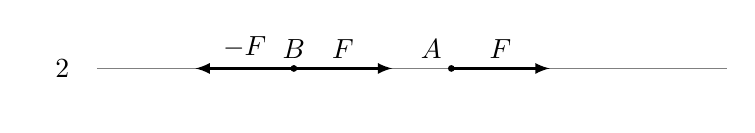
\begin{tikzpicture}
        \coordinate (start) at (-3.5,0);
        \coordinate (end) at (4.5,0);
        \coordinate (a) at (1,0);
        \coordinate (b) at (-1,0);
        \coordinate (len) at (1.25,0);
        \coordinate (nlen) at (-1.25,0);

        \draw[gray, ultra thin] (start) node[anchor=east, inner sep=1em, black] {$\boldsymbol{2}$} -- (end);
        \filldraw[black] (a) node[anchor=south east] {$A$} circle (1pt);
        \draw[black, thick, -latex] (a) -- ++(len) node[black, anchor=south, pos=.5] {$\vect{F}$};
        \filldraw[black] (b) node[anchor=south] {$B$} circle (1pt);
        \draw[black, thick, -latex] (b) -- ++(len) node[black, anchor=south, pos=.5] {$\vect{F}$};
        \draw[black, thick, -latex] (b) -- ++(nlen) node[black, anchor=south, pos=.5] {$-\vect{F}$};
    \end{tikzpicture}

    \begin{tikzpicture}
        \coordinate (start) at (-3.5,0);
        \coordinate (end) at (4.5,0);
        \coordinate (b) at (-1,0);
        \coordinate (len) at (1.25,0);

        \draw[gray, ultra thin] (start) node[anchor=east, inner sep=1em, black] {$\boldsymbol{3}$} -- (end);
        \filldraw[black] (b) node[anchor=south east] {$B$} circle (1pt);
        \draw[black, thick, -latex] (b) -- ++(len) node[black, anchor=south, pos=.5] {$\vect{F}$};
    \end{tikzpicture}
    \caption{}
    \label{fig:forze_equivalenti_elementari}
\end{figure}



\subsubsection{Forze parallele nello stesso verso}

\begin{figure}[!h]
    \centering
    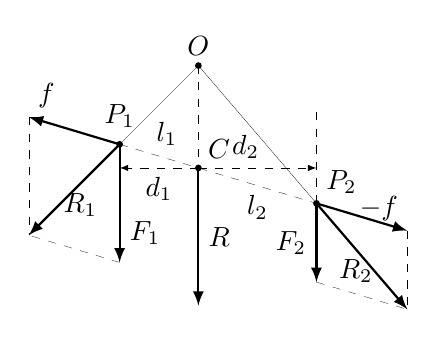
\begin{tikzpicture}
        \coordinate (O) at (0,0);
        \coordinate (P1) at (-1,-1);
        \coordinate (len1) at (0,-1.5);
        \coordinate (P2) at (1.5,-1.75);
        \coordinate (len2) at (0,-1);
        \coordinate (C) at (0,-1.3);

        \filldraw[black] (O) node[anchor=south] {$O$} circle (1pt);

        \filldraw[black] (P1) node[anchor=south, inner sep=6] {$P_1$} circle (1pt);
        \draw[black, thick, -latex] (P1) -- ++(len1)
        node[anchor=west, pos=.75] {$\vect{F}_1$};

        \filldraw[black] (P2) node[anchor=south west] {$P_2$} circle (1pt);
        \draw[black, thick, -latex] (P2) -- ++(len2)
        node[anchor=east, pos=.5] {$\vect{F}_2$};

        \draw[black, ultra thin, domain=0:-1, samples=\tikzsamples] plot (\x, {\x});
        \draw[black, ultra thin, domain=0:1.5, samples=\tikzsamples] plot (\x, {-7/6 * \x});

        \draw[black, ultra thin, dashed] (P1) -- (P2);
        \draw[black, ultra thin, dashed] (P2) -- ++(0,1.25);
        \draw[black, ultra thin, dashed] (O) -- (C);

        \draw[black, ultra thin, dashed, -latex] (C) -- ++(-1,0)
        node[anchor=north, pos=.5] {$d_1$}
        node[anchor=south, inner sep=8, pos=.4] {$l_1$};
        \draw[black, ultra thin, dashed, -latex] (C) -- ++(1.5,0)
        node[anchor=south, pos=.4] {$d_2$}
        node[anchor=north, inner sep=10, pos=.5] {$l_2$};

        \filldraw[black] (C) node[anchor=south west] {$C$} circle (1pt);
        \draw[black, thick, -latex] (C) -- ++(0,-1.75) node[anchor=west, pos=.5] {$\vect{R}$};

        % linee di costruzione R1
        \draw[black, ultra thin, dashed, domain=-1:-28/13, samples=\tikzsamples]
        plot (\x, {-.3 * \x - 2.8});
        \draw[black, ultra thin, dashed] (-28/13,-17/26)
        node[anchor=south west] {$\vect{f}$} -- ++(0,-1.5);
        \draw[black] (-1.5,-1.5) node[anchor=north] {$\vect{R}_1$};

        \draw[black, -latex, thick, domain=-1:-28/13, samples=\tikzsamples] plot (\x, {\x}); % R1

        \draw[black, thick, -latex, domain=-1:-28/13, samples=\tikzsamples] plot (\x, {-.3 * \x - 1.3}); % f

        % linee di costruzione R2
        \draw[black, dashed, ultra thin, domain=1.5:69/26, samples=\tikzsamples]
        plot (\x, {-.3 * \x -2.3});
        \draw[black, dashed, ultra thin] (69/26,-109/52)
        node[anchor=south east] {$-\vect{f}$} -- ++(0,-1);
        \draw[black] (2,-7/3) node[anchor=north] {$\vect{R}_2$};

        \draw[black, -latex, thick, domain=1.5:69/26, samples=\tikzsamples] plot (\x, {-7/6 * \x}); % R2

        \draw[black, thick, -latex, domain=1.5:69/26, samples=\tikzsamples] plot (\x, {-.3 * \x - 1.3}); % -f
    \end{tikzpicture}
    \caption{}
    \label{fig:forze_parallele_stesso_verso}
\end{figure}

\begin{equation*}
    F_1 d_1 - F_2 d_2 = 0
\end{equation*}

\begin{equation}
    \frac{l_1}{l_2} = \frac{d_1}{d_2} = \frac{F_2}{F_1}
\end{equation}



\subsubsection{Baricentro}

Date $n$ forze parallele e orientate nello stesso verso, la posizione della forza risultante
\begin{equation}
    \vect{R} = \sum \vect{F}_i
\end{equation}
sarà determinata dalla condizione che il suo momento rispetto a un generico punto $O$ e la somma dei momenti delle forze abbiano lo stesso valore $\vect{M}$.

\begin{equation*}
    R x_c = F_1 x_1 + \ldots + F_n x_n
\end{equation*}

\begin{equation}
    x_c = \frac{\sum F_i x_i}{\sum F_i}
\end{equation}



\subsubsection{Forze parallele in verso opposto}

\begin{figure}[!h]
    \centering
    \begin{tikzpicture}
        \coordinate (P1) at (0,0);
        \coordinate (P2) at (2,.75);
        \coordinate (C) at (-8/3,-1);

        \filldraw[black] (P1) circle (1pt)
        node[anchor=north west] {$P_1$};
        \draw[black, thick, -latex] (P1) -- ++(0,-1.75)
        node[anchor=east, pos=.5] {$\vect{F}_1$};

        \filldraw[black] (P2) circle (1pt)
        node[anchor=north west] {$P_2$};
        \draw[black, thick, -latex] (P2) -- ++(0,1)
        node[anchor=west, pos=.5] {$\vect{F}_2$};

        \draw[black, ultra thin, dashed, domain=-8/3:2, samples=\tikzsamples] plot (\x, {3/8 * \x});

        \filldraw[black] (C) circle (1pt)
        node[anchor=south east] {$C$};
        \draw[black, thick, -latex] (C) -- ++(0,-.75)
        node[anchor=west, pos=.5] {$\vect{R}$};

        \draw[black, ultra thin, dashed] (C) -- ++(0,2);

        \draw[black, ultra thin, dashed, latex-latex] (C) ++(0,1) -- (P1)
        node[anchor=south, pos=.5] {$d_1$};
        \draw[black, ultra thin, dashed, latex-latex] (C) ++(0,1.75) -- (P2)
        node[anchor=south, pos=.5] {$d_2$};

    \end{tikzpicture}
    \caption{}
    \label{fig:forze_parallele_verso_opposto}
\end{figure}

Il punto $C$ è individuato grazie alla relazione

\begin{equation*}
    -F_1 d_1 + F_2 d_2 = 0
\end{equation*}

\begin{equation}
    \frac{d_1}{d_2} = \frac{F_2}{F_1}
\end{equation}



\subsubsection{Coppia}

Rispetto ad un generico punto $P$ si ha
\begin{equation}
    \begin{split}
        \highlight{ \vect{M} = }
        \vect{M}_1 + \vect{M}_2 & = \vect{OP}_1 \times \vect{F}_1 + \vect{OP}_2 \times \vect{F}_2 = \\
        & = (\vect{OP}_1 - \vect{OP}_2) \times \vect{F}_1 =
        \highlight{ \vect{P_2} \vect{P}_1 \times \vect{F}_1 }
    \end{split}
\end{equation}

\begin{equation}
    M = F_1 d_1 - F_2 d_2 = F (d_1 - d_2) = F b
\end{equation}



\subsubsection{Sollecitazione di un corpo rigido}



\subsection{Corpo girevole intorno a un asse fisso}

\begin{equation}
    M_a = \frac{db_a}{dt}
\end{equation}
\begin{equation}
    b_a = \omega \int_V \rho r^2 \ dV
\end{equation}
prende il nome di \textcolor{accent}{momento d'inerzia assiale} del sistema rispetto ad $a$ l'integrale
\begin{equation}
    \highlight{
        I_a = \int_V \rho r^2 \ dV
    }
\end{equation}

Il momento rispetto a un asse diviene quindi
\begin{equation}
    M_a = I_a \frac{d^2 \varphi}{d t^2} = \pm I_a \frac{d \omega}{dt}
\end{equation}

Attraverso il momento d'inerzia è possibile esprimere facilmente l'energia cinetica di un corpo rigido in rotazione
\begin{equation}
    \highlight{T}
    = \frac{1}{2} \int_V \rho v^2 \ dV = \frac{1}{2} \omega^2 \int_V \rho r^2 \ dV =
    \highlight{
        \frac{1}{2} I_a \omega^2 = \frac{1}{2} I_a \dot{\varphi}^2
    }
\end{equation}

Per una forza $\vect{F}_i$ applicata in $P_i$ il lavoro elementare è
\begin{equation}
    dL_i = \vect{M}_i \cdot \vect{\omega} \ dt
\end{equation}
\begin{equation*}
    dL = \sum \vect{M}_i \cdot \vect{\omega} \ dt = M_a \omega_a dt = M_a \dot{\varphi} dt = M_a d \varphi
\end{equation*}

Per uno spostamento finito il lavoro è definito come
\begin{equation}
    L_{12} = \int_{\varphi_1}^{\varphi_2} M_a (\varphi) d \varphi
\end{equation}
quindi
\begin{equation}
    \highlight{
        d \left( \frac{1}{2} I_a \dot{\varphi}^2 \right) = M_a d \varphi
    }
\end{equation}



\subsection{Momento d'inerzia}

\begin{quote}
    Il momento d'inerzia di un corpo rispetto a un qualsiasi asse ($I_a$) è pari al momento d'inerzia rispetto all'asse parallelo a quello passante per il centro di massa ($I_{a,c}$), aumentato del momento d'inerzia che rispetto all'asse dato avrebbe tutta la massa se fosse concentrata nel centro di massa.
\end{quote}

Indicata con $m$ la massa del corpo e con $d$ la distanza dall'asse si ha

\begin{equation}
    \highlight{I_a = I_{a,c} + md^2}
    \label{eq:teorema_huygens}
\end{equation}



\begin{multicols}{2}
    \subsubsection*{Anello}
    Momento d'inerzia rispetto all'asse dell'anello
    \begin{equation*}
        I_x = m R^2
    \end{equation*}
    Momento d'inerzia rispetto a un diametro
    \begin{equation*}
        I_y = \frac{m R^2}{2}
    \end{equation*}
    Momento d'inerzia rispetto a un asse tangente all'anello
    \begin{equation*}
        I_{y'} = \frac{3mR^2}{2}
    \end{equation*}



    \subsubsection*{Tubo cilindrico}
    Momento d'inerzia rispetto al suo asse
    \begin{equation*}
        I_x = \frac{m}{2} (R_1^2 + R_2^2)
    \end{equation*}



    \subsubsection*{Sbarra cilindrica sottile}
    Momento d'inerzia rispetto a un asse perpendicolare per il punto centrale
    \begin{equation*}
        I_y = \frac{ml^2}{12}
    \end{equation*}
    Momento d'inerzia rispetto a un asse perpendicolare per un estremo
    \begin{equation*}
        I_{y'} = \frac{ml^2}{3}
    \end{equation*}



    \subsubsection*{Parallelepipedo}
    Momento d'inerzia rispetto a un asse per il centro (di massa) e parallelo a uno degli spigoli ($c$)
    \begin{equation*}
        I_x = \frac{m(a^2 + b^2)}{12}
    \end{equation*}



    \subsubsection*{Sfera piena}
    Momento d'inerzia rispetto a un diametro
    \begin{equation*}
        I = \frac{2 m R^2}{5}
    \end{equation*}



    \subsubsection*{Sfera cava a parete sottile}
    Momento d'inerzia rispetto a un diametro
    \begin{equation*}
        I = \frac{2 m R^2}{3}
    \end{equation*}

\end{multicols}



\subsection{Energia cinetica di un corpo rigido}

L'energia cinetica di un corpo rigido è definita dalla somma

\begin{equation}
    \highlight{
        T = \frac{1}{2} m v_c^2 + \frac{1}{2} I_c \omega^2
    }
\end{equation}



\subsection{Leve}

\begin{figure}[!h]
    \centering
    \begin{tikzpicture}

    \end{tikzpicture}
    \caption{}
    \label{fig:leve}
\end{figure}

Perché la leva sia bilanciata rispetto all'asse preso in considerazione i momenti delle forze applicate devono avere come somma nulla

\begin{equation}
    M_1 - M_2 = 0
\end{equation}

\begin{equation}
    \highlight{
        R d_1 = P d_2
    }
\end{equation}